\documentclass[10pt, a5paper]{article}
\usepackage{CJKutf8}

\setcounter{secnumdepth}{1} % levels under \section are not numbered
\setcounter{tocdepth}{2}    % levels under \subsection are not listed in the TOC

%詩套件
\usepackage{verse}
\usepackage{comment}
\usepackage[a5paper,vmargin={15mm,15mm},hmargin={10mm,10mm}]{geometry}

\usepackage{multicol}%多欄套件
\usepackage{graphicx}%圖片套件
%\usepackage{dblfnote}%雙欄註腳

\setlength{\parindent}{2em}
%\setlength{\parskip}{1em}
\renewcommand{\baselinestretch}{1.45}
\setlength\columnsep{2em} % This is the default columnsep for all pages 。兩欄間距

%詩結束的小記
\newcommand{\attrib}[1]{%
\nopagebreak{\raggedleft\footnotesize #1\par}}
\renewcommand{\poemtitlefont}{\normalfont\large\itshape\centering}

\usepackage{blindtext}

\title{龍語筆記小誌 01}
\author{老翰 整理}
\date{2024/01/01 -2024/01/07}

\begin{document}
\begin{CJK}{UTF8}{bsmi}


% ======== 封面標題頁 ========

\maketitle

\thispagestyle{empty} %本頁不要頁碼

%\begin{center}
    %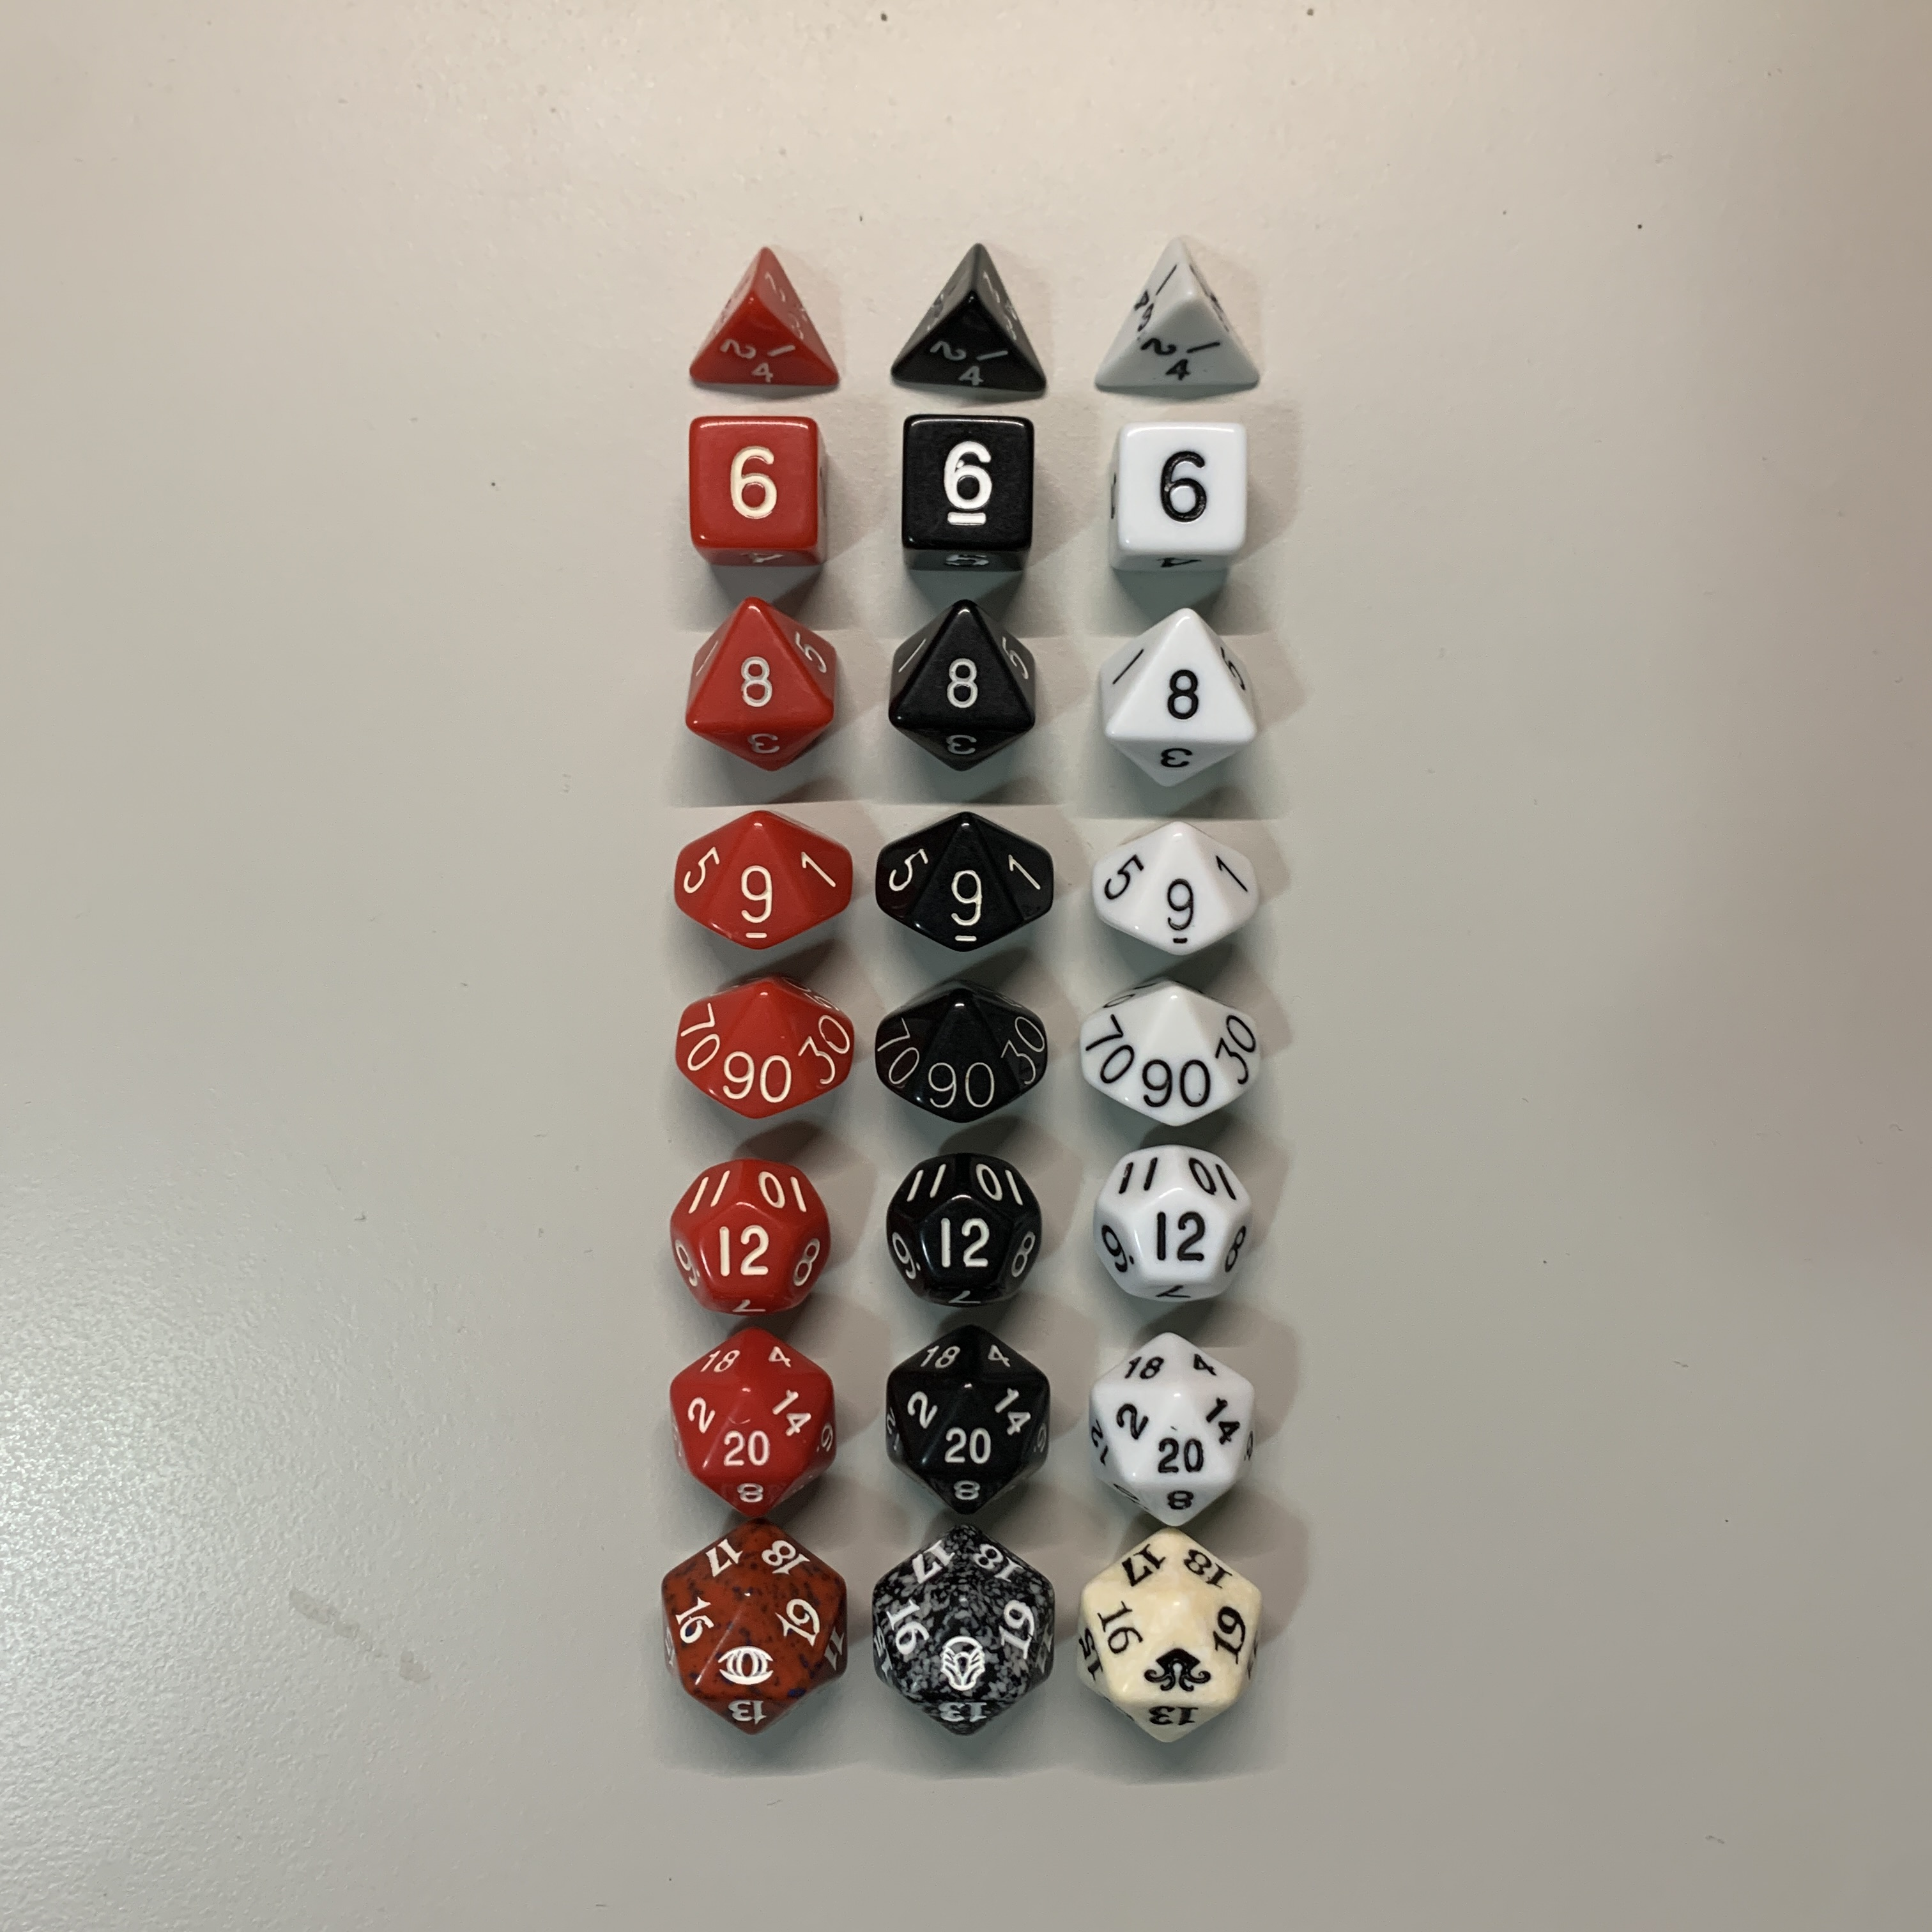
\includegraphics[width=0.9\textwidth]{imgs/zine_issue01_dice2014.jpg}

\begin{figure*}[h]
    \centering
    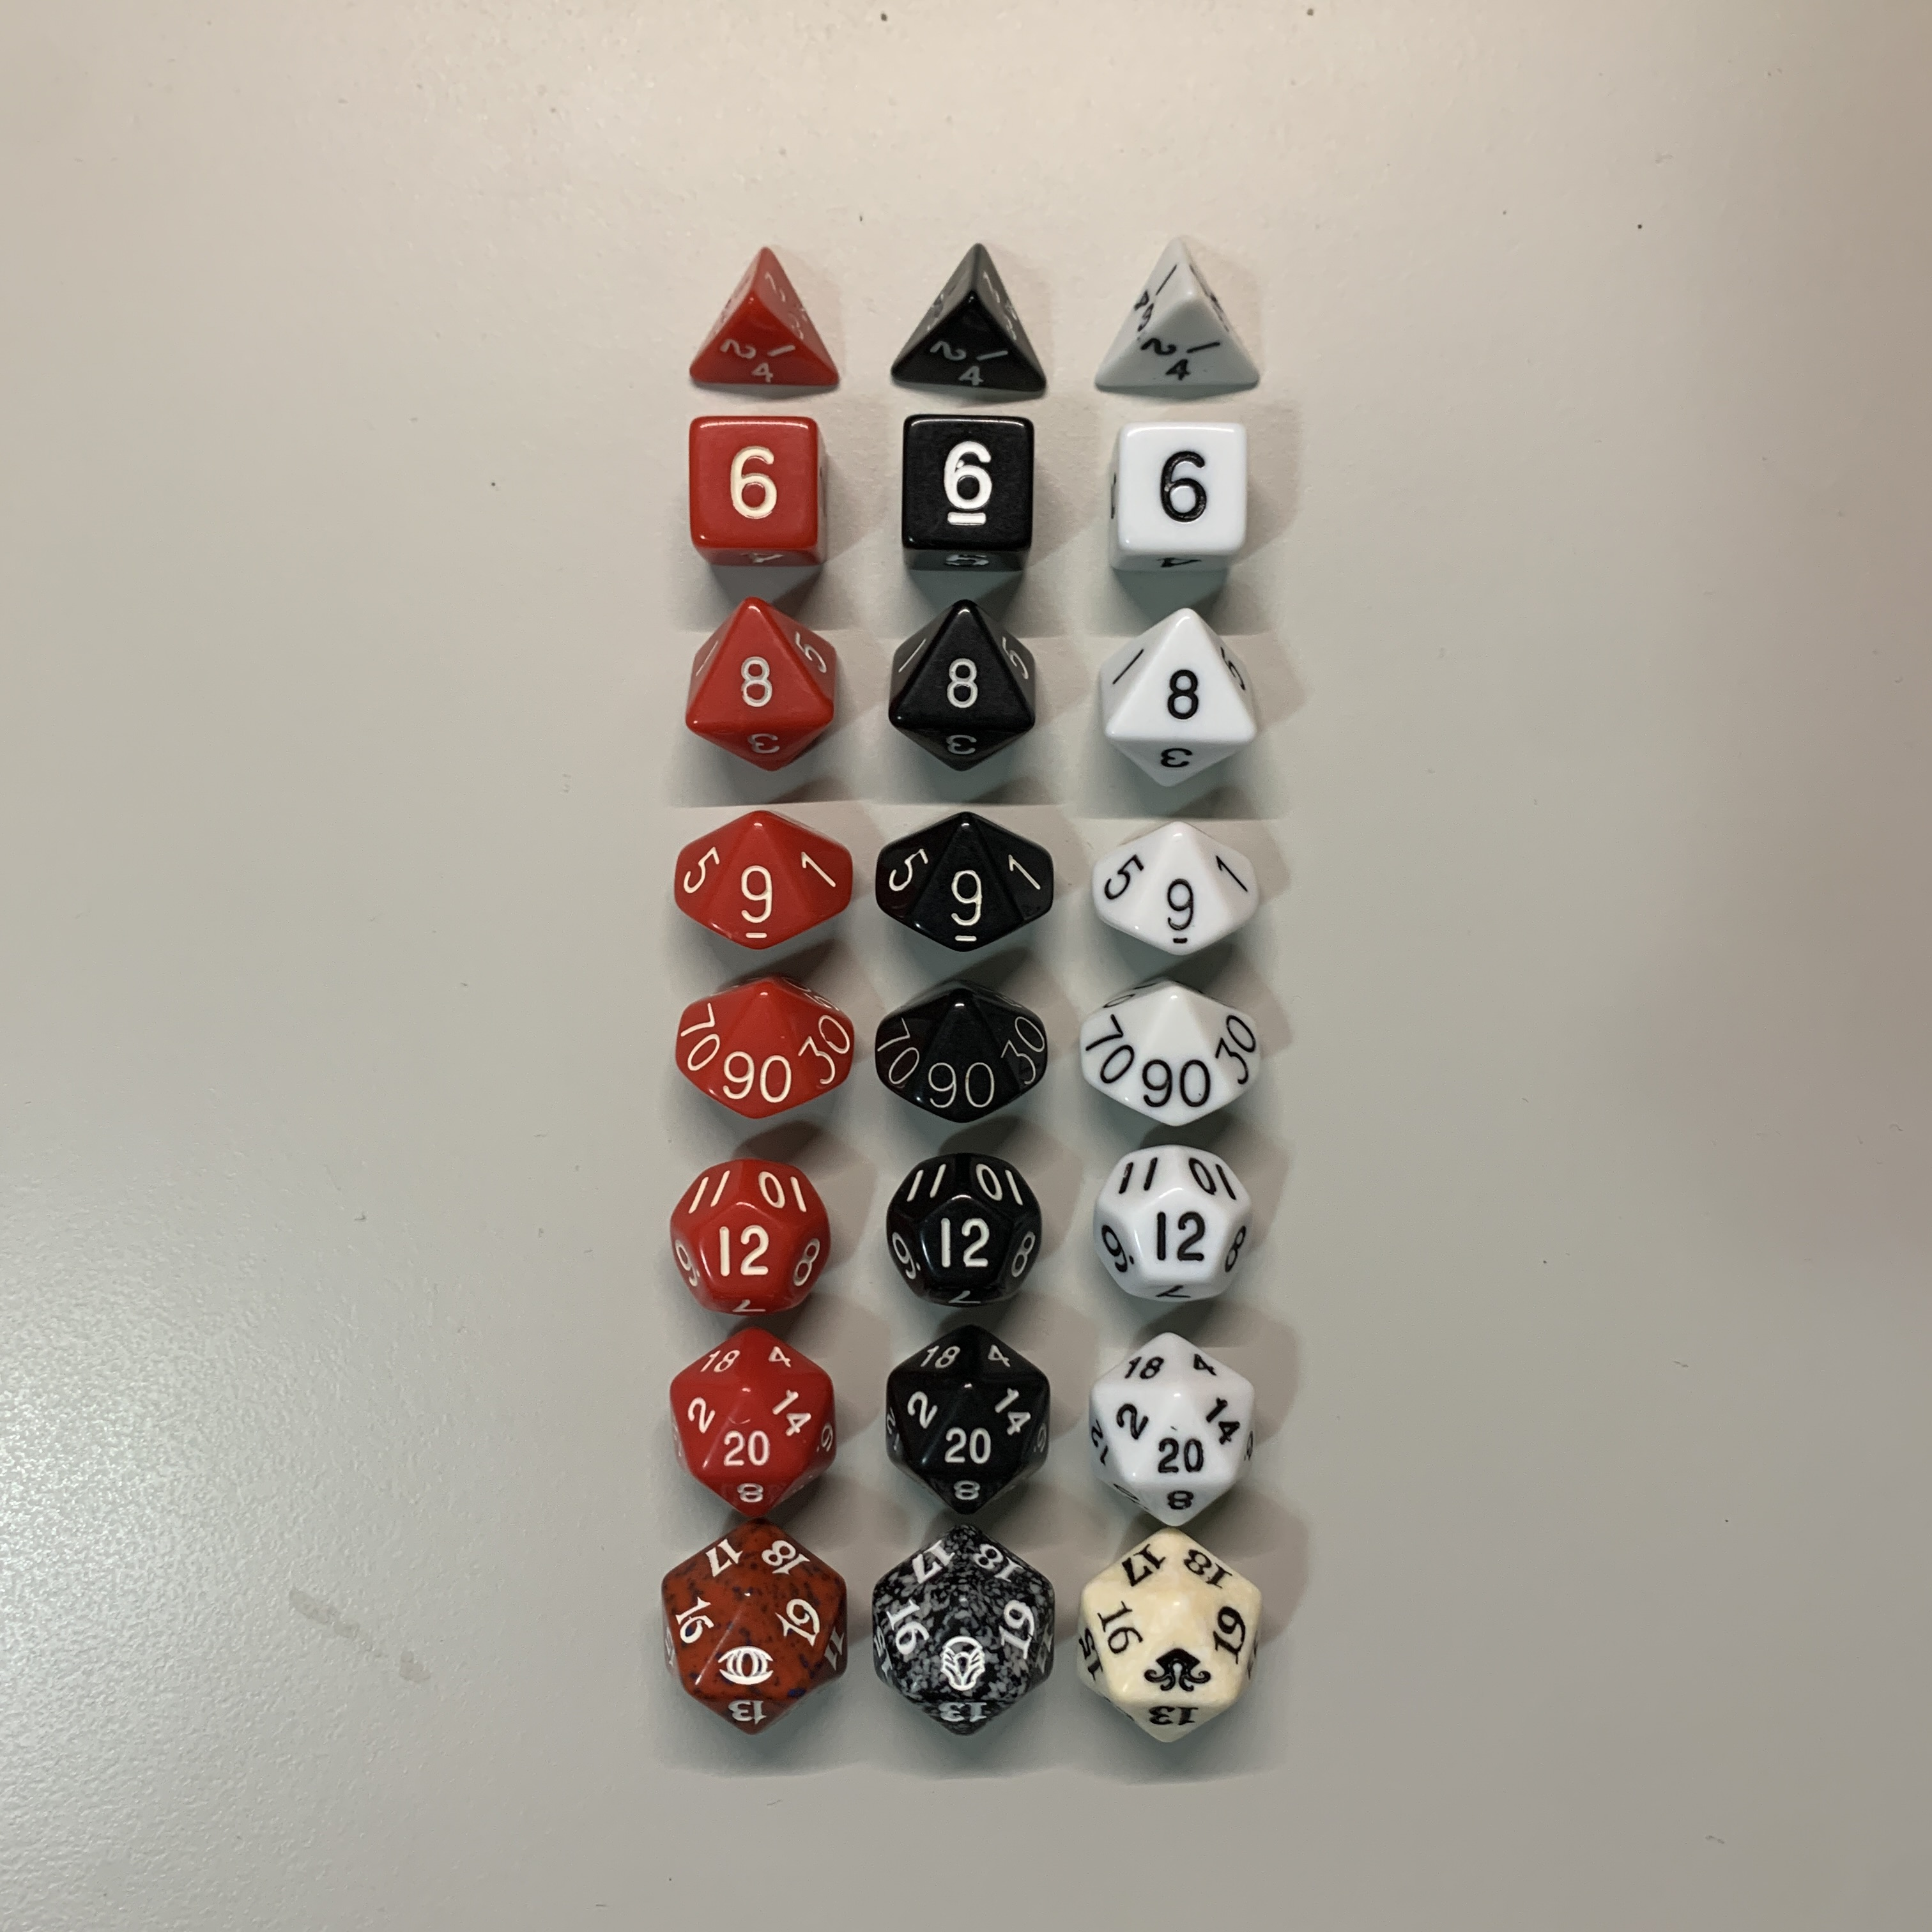
\includegraphics[width=9cm, keepaspectratio]{imgs/zine_issue01_dice2014.jpg}
    \label{fig:封面}
\end{figure*}
%\end{center}

\vfill

\renewcommand{\abstractname}{} %把 abstract 的標題從英文改為中文的「摘要」
\renewcommand{\contentsname}{目錄} %把 tableofcontents 的標題從英文改為中文的「目錄」
\renewcommand{\figurename}{圖} %把 figure 的標題從英文改為中文的「圖」

\begin{abstract}
收錄一些同好每週 TRPG 相關的習作。還有老翰自己關於上一週的筆記。
\end{abstract}

\newcommand{\contactmethod}{
\begin{center}
\noindent\begin{tabular}{|| l ||}
\hline
投稿或相關問題,可以使用以下方式聯絡\\
Email : dragonicnotes@gmail.com\\
\hline
\end{tabular}
\end{center}
}

\pagebreak % 換頁


% ======== 目錄頁 ========

\thispagestyle{empty} %本頁不要頁碼

\tableofcontents % 目錄

\vfill %
\contactmethod

\pagebreak % 換頁


% ========== 2024 ===========


% ========== 第 01 頁 ===========

% ==== 第一週 ====

% \section{第 1 週, 2024/01/01 - 2024/01/07} %章節

\setcounter{page}{1} %從這裡開始第一頁

% ==== 河城紀事 start ====
\section{河城紀事 / 多人協作}

\noindent 專案主持:老翰

\noindent 內容協作:奈羅、江鳥、 RERO 。

\subsection{1/52}

\subsubsection{特殊地點:祭典廣場}

一年一度的河神祭,是這個小城的大事,十二個主要家族的首領唯一會聚集一堂的日子。在河神祭典的表演中,再次確認同盟誓約、無法化解的恩怨可以在此合法決鬥等等。

\subsubsection{都市傳說:戲班的私兵團}

在河城,只有兩種罪,死,或者成為戲子。據說,有受刑人從戲班逃離後,主動投案,選擇接受死刑。據說在舞台周圍藏有各種機關、舞台後的戲班居住地則是僅次於領主內城的軍火庫。

\subsubsection{NPC :戲班老闆}

烏首.星落( Blackhead Starfall ),戲班老闆。戲班的人尊稱他為「頭兒」。星落這個姓氏,知道這個地方的歷史的人,就知道是「星樂埕」的原始發音,但後來被用作「分家」或者被逐出家族者的姓氏。

\subsubsection{奇特物品:河神的酒杯}

據說用這支酒杯,盛裝上好的酒倒入河中,能夠平息河神的怒氣。遠古時代、在戰亂、更暴力的年代,據說是以敵人的血祭神。

\vfill
\pagebreak

\subsection{討論記錄摘要}

這個小節打算用來記錄討論的過程,但怎麼樣摘要討論過程還沒有非常明確的做法,希望一月能慢慢理出一個頭緒。

\begin{figure*}[h]
    \centering
    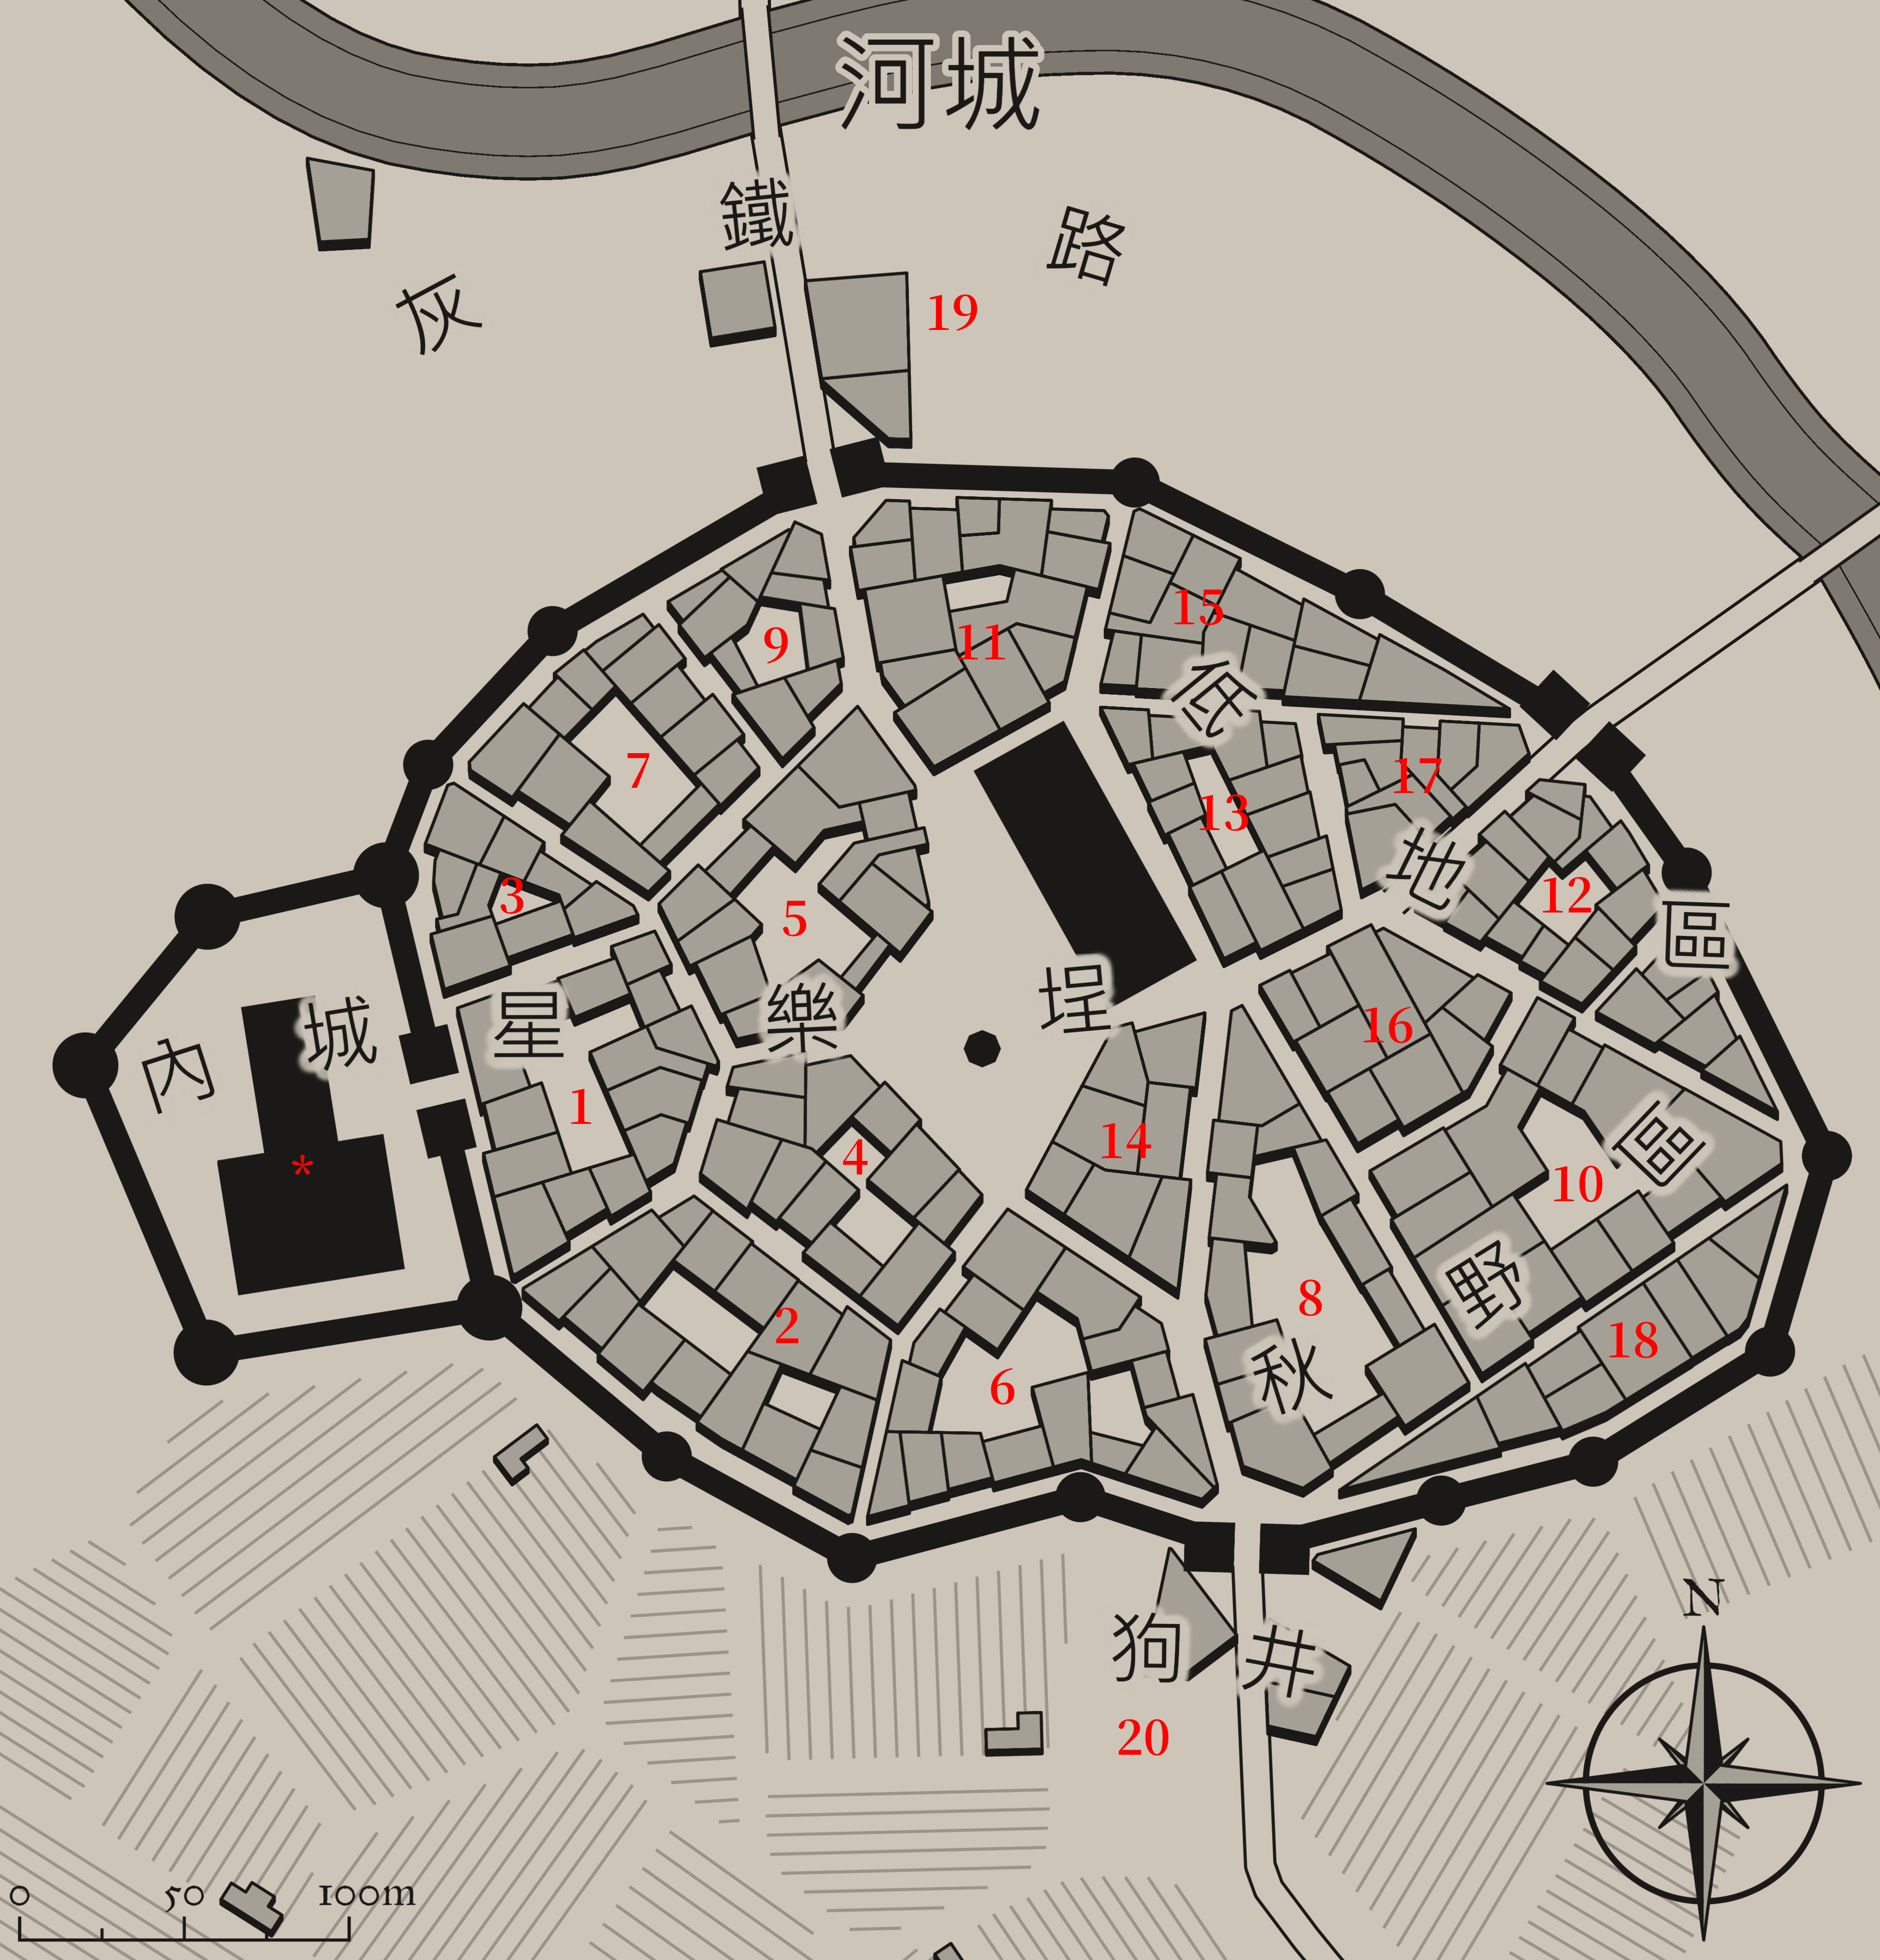
\includegraphics[width=9cm, keepaspectratio]{imgs/RiverCity_v01.jpg}
    \caption{第一週河城地圖}
    \label{fig:2024W01}
\end{figure*}

Dungeon23 我撐不到一個月就放棄了。但 2024 年還是打算試著寫點東西到年底,覺得一週為單位來做比較可以達成。可能因為去年帶完《深水城:龍金劫》的關係,我想要寫一個「城市」相關的跑團資料的創作集。先用產生器\footnote{https://watabou.github.io/city.html }產生了一張初步的地圖,協助發想,之後也許有機會再重新繪製。

在我自己的 Discord 伺服器和 Level 1 Game Jam 的伺服器都開了專案,稍微貼了點初步的構想資料,有些同好有興趣一起創作。我會在此整理、收錄大家創作的成果,可以的話會記錄這個共同創作的過程。


原本預計年末產出:

\begin{itemize}
  \item 52個特殊地點
  \item 52個都市傳說
  \item 52個NPC
  \item 52個奇特物品
\end{itemize}

本來只是想自己一個人慢慢寫,但有同好加入之後覺得可以擴大產出的內容。我自己的部分至少是完成上述的一周一組的部分(小標題為 X/52 ),其他共同創作的東西會盡量一起收錄。

目前大概討論出來的部分是,河城(之後也許要再想個名字),原本是個軍事屯墾單位,氣候的ˋ部分參考我們生活的亞熱帶,每年夏季有機會發生超大暴風挾帶豪雨( aka 颱風)所以有對屋子的堅固性要求跟風暴系列神祉在這裡是主要的信仰的特色。會從台灣以前有城牆的城市找參考資料,例如台北、台南、新竹(竹塹)、彰化縣城等。有十二個最早的家族,想用天干地支的概念去寫東西。

某種逃難或者侵略者的先遣隊,但是大後方發生變動而與原本的國家失去聯繫或後備支援而必須在此地屯墾。隨著時間過去,原本的軍事要塞小鎮,與附近的地區貿易,漸漸擴大規模,可能需要重繪地圖,變成有兩環或三環外城的大一點的城市。詳細的創作可能會參考佛羅倫薩與巴黎,有一條河流穿過城市的情況,待之後詳細討論。

\subsection{附記}

在討論的過程中,我們或多或少從發生在台灣的一些故事或資料、文獻、遺跡等等取得一些靈感,這個創作的東西都是虛構無特別想影射任何事物或人,對於生活在這塊土地上的人們的族群、文化與信仰都無不敬之意,如果有任何文字或者引用的東西造成困擾,請不吝來信指正。

\attrib{老翰 2024.01.10}


\vfill
\pagebreak % 換頁
% ======== 附記結束 ========
% ==== 河城紀事 end ====



% ======== NPC24 ========

\section{NPC24 / 加島} 

作者:加島

\subsection{蜜爾娜}

\textbf{生命骰: 9}\\
\textbf{防禦等級:} –8[27]\\
\textbf{攻擊:}電擊(2d6)\\
\textbf{移動:}18\\
\textbf{豁免:}6\\
\textbf{士氣:}12\\
\textbf{陣營:}秩序\\
\textbf{挑戰等級/經驗值:}11/2400\\

凡到過南方的人,都會告誡最好在晚上遠離沼澤,那些潛伏在裏頭的魔物大多是女巫法術下的犧牲品。有些僥倖逃出生天的人則述說他們看見一團翠綠色、有著成年女性外觀的火光,據說那是沼澤女巫最年長,也曾是最鍾愛的女兒,即使在死後依舊頑強抵抗她的魔法。如果不幸身陷沼澤,被黑暗包圍的時候可以試著呼喊她的名字—蜜爾娜,或許可以尋得一線生機。\footnote{本篇獲得作者授權轉載。作者說明:「目前的我流規則只有:每週寫一個NPC,不限題材與系統。預計每隔一陣子換一個系統。」原文連結: https://www.plurk.com/p/pi7nk8}\\

\noindent \textbf{蜜爾娜}: 生命骰 9; 防禦等級 –8[27]; 攻擊:電擊(2d6); 移動 18; 豁免 6; 士氣 12; 陣營:秩序; 挑戰等級/經驗值 11/2400\\

\noindent 系統: Swords \& Wizardry Complete\footnote{https://preview.drivethrurpg.com/en/product/438315/Swords--Wizardry-Complete-Rulebook-Revised}/OD\&D


\vfill
\pagebreak
% ======== NPC24 end ========



% ======== 社群觀察 ========
\section{網路觀察與閱讀摘要}

主筆:老翰

筆者嘗試從噗浪、 fb 、推特這三個社群網站觀察一些 TRPG 的社群或貼文,寫一些摘要。可能不見得每週都有重要的事情要記錄,但試著記錄看看。

\begin{itemize}
  \item The MCDM RPG 群眾募資結束,共募得 4,600,520 USD 。 2024/01/05 , 4:01pm , UTC+8 。\footnote{https://www.backerkit.com/c/projects/mcdm-productions/mcdm-rpg}
  \item Humble Bundle 出現了 Call of Cthulhu 7th 的 Bundle 。這是一個非常不錯的 Bundle\footnote{https://www.humblebundle.com/books/call-cthulhu-chaosium-inc-books} ,如果有想擁有 CoC7 的規則書電子書的人,這是個好機會。此 Bundle 收錄的書本書名記錄如下:
  \begin{itemize}
    \item Call of Cthulhu: Investigator Handbook
    \item Call of Cthulhu: Keeper Screen Pack
    \item Pulp Cthulhu
    \item Malleus Monstrorum
    \item Dead Light and Other Dark Turns
    \item A Cold Fire Within
    \item Berlin The Wicked City
    \item Down Darker Trails
    \item Cthulhu Dark Ages 3rd Ed
    \item Reign of Terror
    \item Mansions of Madness Vol. 1
    \item Petersen's Abominations
    \item Alone Against the Tide
    \item Alone Against the Frost
    \item Does Love Forgive?
    \item Call of Cthulhu: Keeper Rulebook
    \item Gateways to Terror
    \item Grand Grimoire of Cthulhu Mythos Magic
    \item Keeper Tips
    \item Alone Against the Dark
    \item Malleus Monstrorum Keeper Deck
    \item Call of Cthulhu Starter Set
    \item Doors to Darkness
    \item Petersen Guide to Lovecraftian Horrors
    \item Call of Cthulhu the Coloring Book
  \end{itemize}
\end{itemize}

\vfill
\pagebreak
% ======== 社群觀察 end ========


封面圖是老翰 2014 剛開始玩 TRPG 的時候用的套骰,魔法風雲會的 d20 只是剛好有相近的顏色,後來拿來補充玩 dnd5e 的時候有 2d20 比較方便。

\section{徵稿}

\begin{itemize}
  \item 封面圖
  \item 純文字文章,包含標點符號,全形字最少 140 字,最多不超過 1800 字。
  \item 其他圖片、文字等等關於 TRPG 的在這個小誌分享的內容
\end{itemize}



\vfill
\contactmethod
\pagebreak

% ======== 本文件 end ========


\begin{comment} 
%貼詩用的一些格式
===========================================
\subsection{}
\begin{verse}

\end{verse}
\attrib{}
\pagebreak

\section{} %章節
\pagebreak  %章節

\pagebreak %長詩手動換頁


\vfill %註腳
\footnotetext{} %註腳

===========================================

\noindent\rule{\textwidth}{1pt} %切分整頁的直線

===========================================
\end{comment} 

\end{CJK}
\end{document}